\documentclass{article}
\usepackage[utf8]{inputenc}
\usepackage{graphicx}
\graphicspath{ {img/} }

\title{Universidad Nacional Aut\'onoma de M\'exico\\
Facultad de Ciencias\\
Lenguajes de Programación \\
Tarea 1}
\author{Luna Vázquez Felipe Alberto}
\date{Fecha de entrega: 14 de Agosto del 2018.}

\begin{document}

\maketitle

\section{Kathleen Booth}
El Laboratorio de Computaci\'{o}n de el Departamento de Inform\'{a}tica fundado por Andrew Booth que se vio involucrado en calculadoras autom\'{a}ticas durante la Segunda Guerra Mundial, al mismo tiempo que trabajaba en la determinaci\'{o}n de estructuras cristalinas usando datos de difracci\'{o}n de rayos X. Kathleen Britten 
naci\'{o} en Strourbridge, Inglaterra, concluy\'{o}  su licenciatura en matem\'{a}ticas de la Universidad de Londres en 1944 y m\'{a}s tarde su doctorado en Matem\'{a}ticas Aplicadas en 1950. \newline

Kathleen como asistente y pr\'{o}xima esposa de Andrew se propuso construir la que ser\'{\i}a la primera computadora de la universidad, en 1946. Un a\~{n}o m\'{a}s tarde ambos viajaron al Instituto de Estudios Avanzados en Princeton,E.U donde trabajaron con el gran John Von Neumann quien los convenci\'{o} de implementar su conocida arquitectura en la calculadora autom\'{a}tica de retransmisi\'{o}n (ARC) que estaban construyendo. Claramente obtuvieron avances y publicaron un sonado documento titulado  "consideraciones generales en el dise\~{n}o de una computadora electr\'{o}nica multiuso". \newline

Kathleen siempre se interes\'{o} en las m\'{a}quinas dise\~{n}adas por Andrew, de 1947 a 1953, construyeron tres m\'{a}quinas: ARC (computadora de retransmisi\'{o}n autom\'{a}tica), SEC (computadora electr\'{o}nica simple) y APEC (computadora electr\'{o}nica de uso m\'{u}ltiple), Andrew constru\'{\i}a las m\'{a}quinas y Kathleen las programaba. Conseguir su funcionamiento implicaba la prueba de el ordenamiento de los componentes electr\'{o}nicos, adem\'{a}s de verificar que el programa se ejecutara correctamente. \newline

Kathleen desarrollo un lenguaje ensamblador para sus computadoras, el que es considerado el primero de su clase y en 1958 public\'{o} un libro sobre software titulado \textquotedblleft{}Programaci\'{o}n para una calculadora digital autom\'{a}tica\textquotedblright{}.  Su computadora m\'{a}s conocida APEC fue dise\~{n}ada en 1949 y tal fue su ejemplo que la empresa British Tabulating Machine Company (BTM), quien fabricaba y vend\'{\i}a m\'{a}quinas de procesamiento de datos que durante la Segunda Guerra Mundial algunas se usaron para romper las cifras de la m\'{a}quina alemana enigma, us\'{o} sus circuitos como base para construir algunas de sus mejores m\'{a}quinas. \newline

En 1957, Kathleen fund\'{o}  la escuela de inform\'{a}tica  y Sistemas de Informaci\'{o}n en el colegio Birkbeck (Universidad de Londres). En los siguientes a\~{n}os, el Departamento creci\'{o} y hubo un flujo constante de revistas y documentos de conferencias y, en particular, una serie de libros, varios de ellos en m\'{a}s de una edici\'{o}n. Un hito notable fue el libro de Kathleen Booth sobre la programaci\'{o}n de computadoras APEC. \newline

Despu\'{e}s de su tiempo en Birkbeck, Kathleen se mud\'{o} a Canad\'{a}, donde se convirti\'{o} en Investigadora y profesora, primero en la Universidad de Saskatchewan y de Matem\'{a}ticas en la Universidad de Lakehead. Su investigaci\'{o}n en redes neuronales condujo a simulaciones exitosas de c\'{o}mo los animales reconocen patrones. \newline

El principal logro de  Kathleen en el \'{a}rea de las ciencias de la computaci\'{o}n fue la creaci\'{o}n de el primer lenguaje ensamblador, que en aquel entonces lo cre\'{o} para programar sus m\'{a}quinas pero que fue la base para dar pie a los lenguajes de programaci\'{o}n m\'{a}s actuales. \newline

Claramente  Kathleen es un personaje muy importante en el \'{a}rea de las ciencias de la computaci\'{o}n, considerando los pocos recursos tecnol\'{o}gicos de ese tiempo y que a\'{u}n no se ten\'{\i}a formalmente el concepto de la computadora, logr\'{o} influir altamente en este.
\newline

Bibliograf\'{\i}a:

- University of London,https://www.dcs.bbk.ac.uk/about/our-history/,Consultado el d\'{\i}a: 12/08/2018

-  University of London,School of Computer Science \& Information Systems
A Short History,Consultado el d\'{\i}a: 12/08/2018



\section{Digr\'afica}

\newline
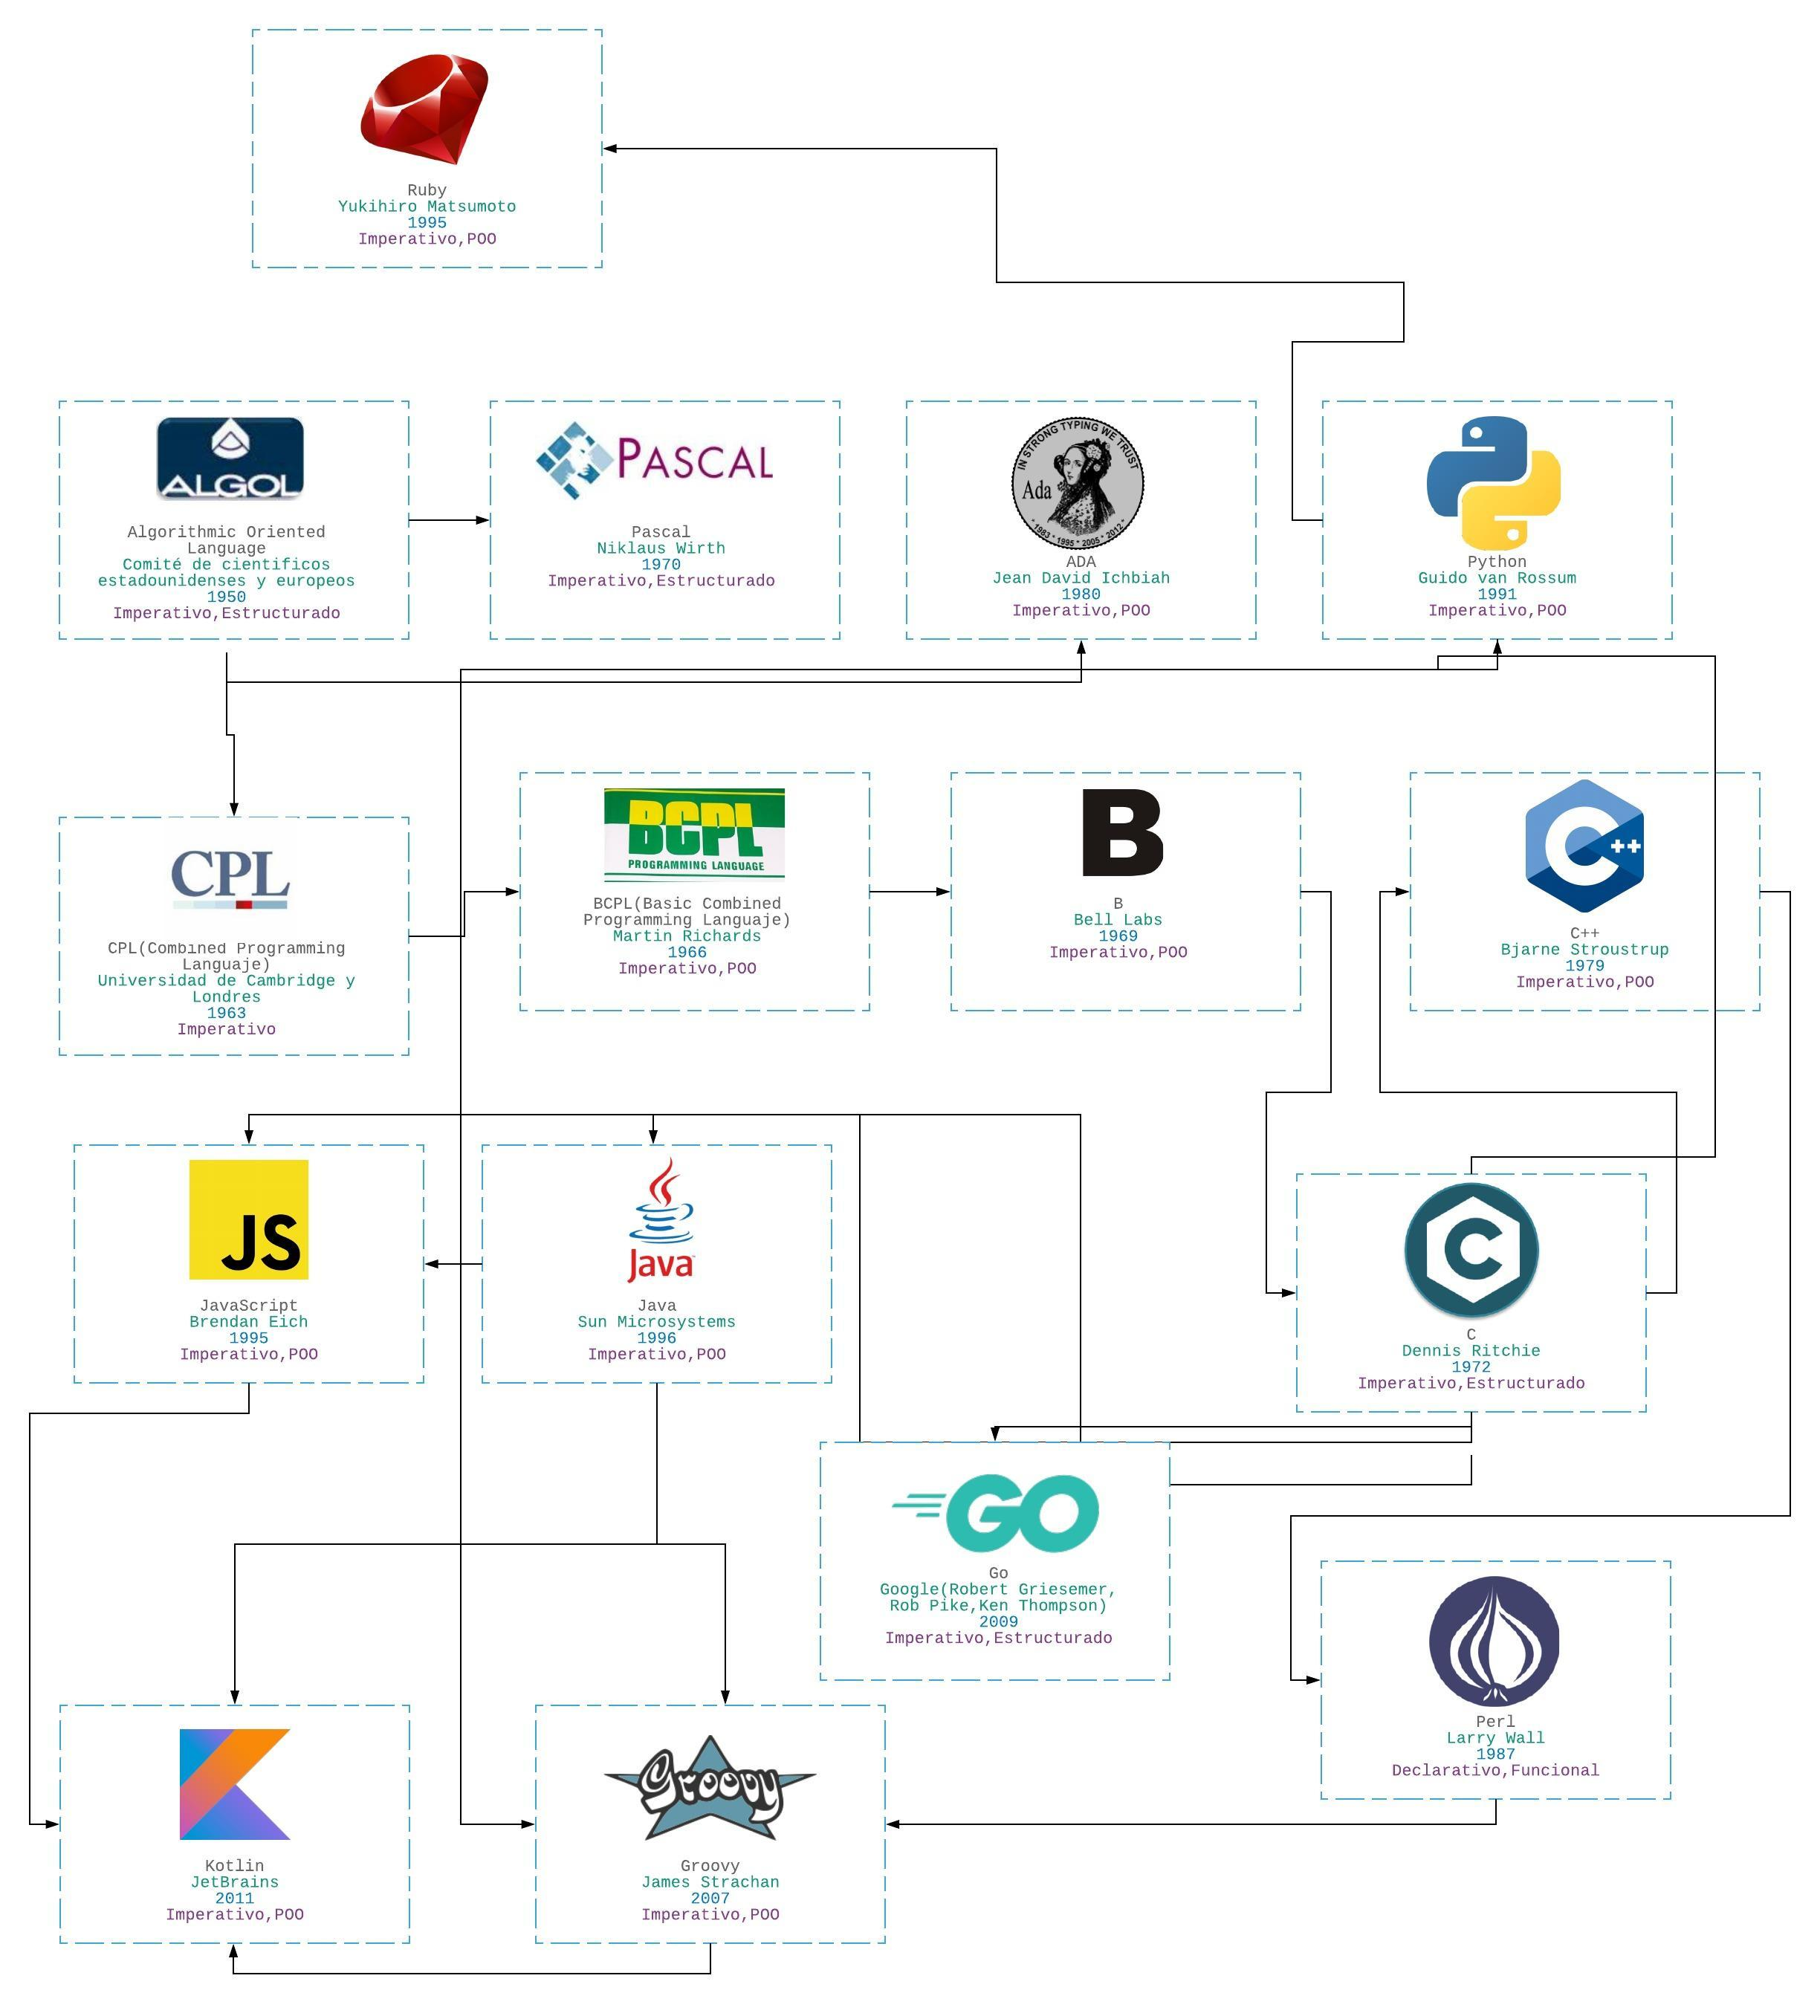
\includegraphics[scale=0.4]{Diagrama_Lenguajes}

\newpage

\section{Lenguajes "multiparadigma"}

1. \textquestiondown{}Por qu\'{e} se dice que un lenguaje es multiparadigma?


Se dice que un lenguaje es multiparadigma cuando estos permiten crear \textquotedblleft{}programas usando m\'{a}s de un estilo de programaci\'{o}n\textquotedblright{}, seg\'{u}n lo define Bjarne Stroustrup, creador del lenguaje C++.


2. \textquestiondown{}Existe el paradigma multiparadigma?
En mi opini\'{o}n no existe tal, ya que un paradigma de programaci\'{o}n es una forma espec\'{\i}fica de resolver un problema y ser\'{\i}a muy complicado resolver este si se trata de hacer de diferentes maneras a la misma vez, por el contrario, si estoy de acuerdo con que un programa pueda implementar diferentes paradigmas y tener varias opciones de como resolver un problema dentro de un mismo lenguaje.



\end{document}

